%%% Esqueleto base de la presentacion
%%% No agregar las paginas con un include
%%% Lo que quieran aportar deben ser usuarios del TRAC

\documentclass{beamer}
\usepackage[spanish,activeacute]{babel}
\usepackage[utf8]{inputenc}
\usepackage{listings}
\usepackage{color}
\usepackage{url}
\usepackage{graphics}
\definecolor{gray2}{rgb}{100,100,100}

\usetheme[pageofpages=of,% String used between the current page and the
                         % total page count.
          alternativetitlepage=true,% Use the fancy title page.
          titlepagelogo=img/logo,% Logo for the first page.
          watermark=img/di-off,% Watermark used in every page.
          watermarkheight=100px,% Height of the watermark.
          watermarkheightmult=4,% The watermark image is 4 times bigger
                                % than watermarkheight.
          ]{Torino}

\usecolortheme{nouvelle}

\author{\normalsize
\textbf{Integrantes:}\\
Rodrigo Fernández\\
Ignacio Villacura\\
Gabriel Zamora\\
Cristian Maureira\\
\textbf{Jefe de Proyecto:}\\
Esteban Bombal\\
\textcolor{gray}{tsc@csrg.inf.utfsm.cl}
}

\title{\Huge Control de Acceso Lógico}
\subtitle{\Large \textit{``Presentación Final''}}
\institute{Universidad Técnica Federico Santa María}
%\date{\today}

\begin{document}
\begin{frame}[t,plain]
\titlepage
\end{frame}


\section{Resumen}

\frame{
\frametitle{Resumen}

Implementación de un framework de seguridad basado en Java, llamado \textbf{JAAS}. 
Establecer una conexión a servicios de directorios mediante \textbf{LDAP} para la conexión a la máquina \textbf{JBoss} correspondiente.

}

\section{Organización}
% Explicar el metodo de trabajo

\frame{
\frametitle{Organización}
\framesubtitle{Medios de comunicación}
\begin{itemize}
	\item Skype
	\item Alias de Correo
	\begin{itemize}
		\item tsc@csrg.inf.utfsm.cl
	\end{itemize}
	\item TRAC
	\begin{itemize}
		\item \url{http://trac.inf.utfsm.cl/proyectos/tsc\_02/}
	\end{itemize}
\end{itemize}

}

\frame{
\frametitle{Organización}
\framesubtitle{Cargos}
\begin{itemize}
	\item Jefe de Proyecto
	\begin{itemize}
		\item Esteban Bombal
	\end{itemize}
	\item Área Documentación
	\begin{itemize}
		\item Rodrigo Fernández y Cristián Maureira
	\end{itemize} 
	\item Área Técnica
	\begin{itemize}
		\item Ignacio Villacura y Gabriel Zamora
	\end{itemize}
\end{itemize}

}


\section{Acerca}
% Algunas definiciones para que se entienda el coontenido

\frame{
\frametitle{Acerca}
\framesubtitle{Objetivos}
\begin{itemize}
	\item Instalación de API JAAS
	\item Integración de LDAP en JBoss usando JAAS
	\item Integración de JAAS en Tomcat
	\item Implementación de Single Sign-On
\end{itemize}
}

\frame{
\frametitle{Acerca}
\framesubtitle{Conceptos}
\textbf{JAAS}
\begin{itemize}
	\item Java Authentication and Authorization Service
	\item Interfaz de Programación de Aplicaciones
	\item Permite a las aplicaciones Java acceder a servicios de control de autenticación y acceso.
\end{itemize}
}

\frame{
\frametitle{Acerca}
\framesubtitle{Conceptos}
\textbf{JBoss}
\begin{itemize}
	\item Es un servidor de aplicaciones J2EE de código abierto implementado en Java puro.
	\item Como es basado en Java, puede ser utilizado en cualquier SO que lo soporte.
	\item Implementa todo el paquete de servicios de J2EE.
\end{itemize}
}

\frame{
\frametitle{Acerca}
\framesubtitle{Conceptos}
\textbf{SSO}
\begin{itemize}
	\item Single Sign-On o Reduced Sign-on Systems
	\item Procedimiento de autenticación
	\item Habilita al usuario para acceder a varios sistemas con una sola instancia de identificación.
	\item Hay cinco tipos principales de SSO:
	\begin{itemize}
		\item Enterprise Single Sign-On (E-SSO)
		\item Web Single Sign-On (Web-SSO)
		\item Kerberos
		\item Identidad Federada
		\item OpenID
	\end{itemize}
\end{itemize}
}


\frame{
\frametitle{Acerca}
\framesubtitle{Conceptos}
\textbf{Servlet}
\begin{itemize}
	\item Objetos que corren dentro de un contenedor de servlets (ej: Tomcat) y extienden su funcionalidad.
	\item También dentro de un servidor de aplicaciones.
	\item ...además tendrá contenedor para objetos más avanzados (ej: EJB).
\end{itemize}
}


\section{Desarrollo}
 %Explicar lo que se hizo

\frame{
\frametitle{Análisis}
\framesubtitle{Instalación API JAAS}
\begin{itemize}
	\item Primer paso.
	\item Más importante para poder realizar todas las configuraciones restantes.
	\item Necesariamente funcional.
\end{itemize}
}

\frame{
\frametitle{Análisis}
\framesubtitle{Integración de LDAP en JBoss usando JAAS}
\begin{itemize}
	\item JBoss con el módulo LoginLdapModule
	\item Configuración módulo para autentificación y autorización mediante JAAS.
\end{itemize}
}

\frame{
\frametitle{Análisis}
\framesubtitle{Integración de JAAS en Tomcat}
\begin{itemize}
	\item Es posible utilizar JAAS como mecanismo de autenticación.
	\item Se pierde flexibilidad una vez autenticado el usuario.
	\item ...aplicación web es otro contexto.
	\item Necesidad de implementar servlets en la implementación de JAAS.
	\item ...con el fin de reforzar control de acceso.
\end{itemize}
}

\frame{
\frametitle{Diseño}

\begin{itemize}
	\item Objetivo principal, acceso a diferentes tipos de sistemas con JAAS (y SSO).
	\item Único Login
	\item ...luego se le asigna rol.
	\item Finalmente el usuario obtiene los permisos necesarios para acceder a aplicaciones
\end{itemize}
}

\frame{
\frametitle{Diseño}
\begin{center}
	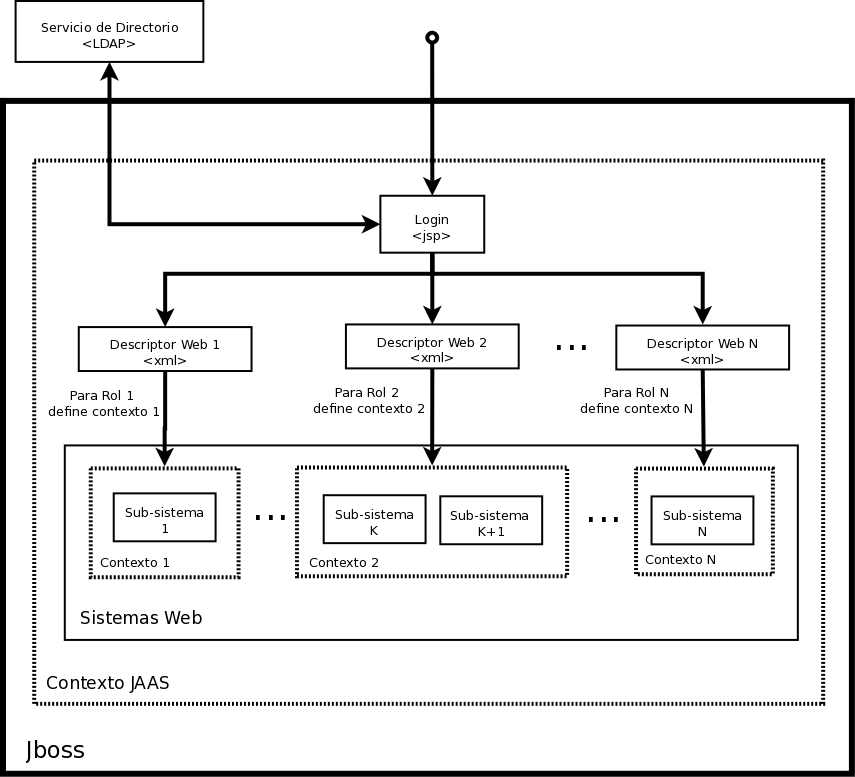
\includegraphics[width=0.7\textwidth]{../reporteTecnico/img/diseno.png}
\end{center}
}

\frame{
\frametitle{Implementación}
\framesubtitle{Instalación de base de datos LDAP}
\begin{itemize}
	\item Bajar e instalar OpenLDAP
	\item Configurar slapd.conf (suffix, rootdn, rootpw, etc)
	\item Tener Usuarios y Grupos que serán usados en JBoss
\end{itemize}
}

\frame{
\frametitle{Implementación}
\framesubtitle{Implementación del SSO en JBoss}
\begin{itemize}
	\item Edición de archivo de configuración en JBoss (server.xml)
\end{itemize}
}

\frame{
\frametitle{Implementación}
\framesubtitle{Integración de LDAP usando JAAS sobre JBoss}
\begin{itemize}
	\item JBoss usa LoginLdapModule para conectarse con LDAP.
	\item Edición de archivo login-config.xml
	\item Conectarse mediante aplicación JAAS (Servlet) 
\end{itemize}
}


\section{Conclusiones}
% Conclusiones del trabajo

\frame{
\frametitle{Conclusiones}
\framesubtitle{Pruebas}
\begin{itemize}
	\item Se realizaron en el servidor JBoss con JAAS y SSO.
	\item Verificar funcionalidad, servlet en el servidor Tomcat (user y pass)
\end{itemize}
}

\frame{
\frametitle{Conclusiones}
\framesubtitle{Resultados}
\begin{itemize}
	\item Los resultados obtenidos son varios.
	\item Habilitar autentificación vía JAAS en un servidor JBoss.
	\item Autentificar contra LDAP al igual que utilizara el SSO para sesiones independientes.
	\item Lo único que no se llevo cabo fue la integración con los demás grupos.
\end{itemize}
}

\frame{
\frametitle{Conclusiones}
\framesubtitle{Logros}
\begin{itemize}
	\item Independiente de la falta de integración...
	\item se usaron todos los servicios que se requerían, LDAP, Tomcat y JBoss.
	\item Configuración de JAAS y SSO fue bastante simple en el servidor JBoss.
	\item Implementación compleja del servlet que integra todo lo visto.
	\item JAAS es una herramienta bastante útil en cuanto a Control de Acceso Lógico.
	\item ...y con Single Sign-On, sistema aún más robusto.
\end{itemize}
}


\section{Agradecimientos}
% Agradecimientos al labcomp, csrg, etc

\frame{
\frametitle{Agradecimientos}
\begin{itemize}
	\item Laboratorio de Computación (LabComp), DI, UTFSM
	\item Computer Systems Research Group (CSRG), DI, UTFSM
\end{itemize}
}


\end{document}
